\begin{figure}%[t]
%  \center
  \vspace{-0.5cm}
\begin{tabular}{ccc}
% \hspace{-3cm}\panel{A} & \\[-0.6cm]
% % \\[-0.6cm]
  % \multicolumn{2}{c}{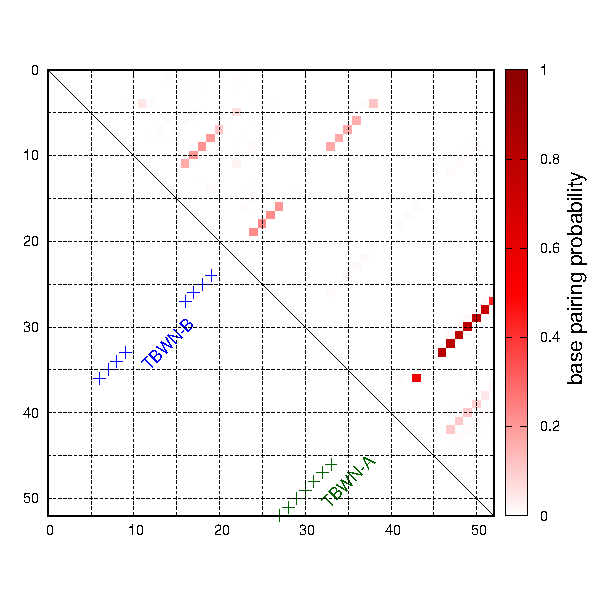
\includegraphics[scale=0.7]{figs/heatmap_fig1A}}
  \\[-0.1cm]  
  \hspace{-.3cm}
  \raisebox{1.7cm}{\panel{A}}
  \hspace{-.3cm}
  %\hspace{-3.5cm}
  \raisebox{-1.cm}{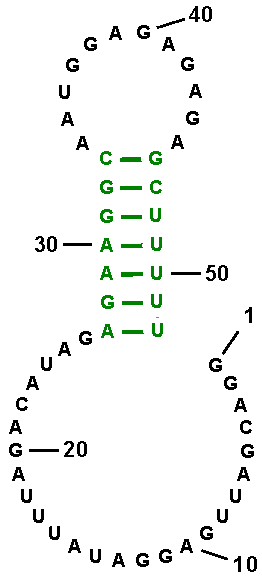
\includegraphics[scale=0.3]{figs/TBWN-A-3}}
  &
  \hspace{.0cm}\raisebox{.8cm}{\panel{B}}
\raisebox{-2.2cm}{\hspace{-.7cm}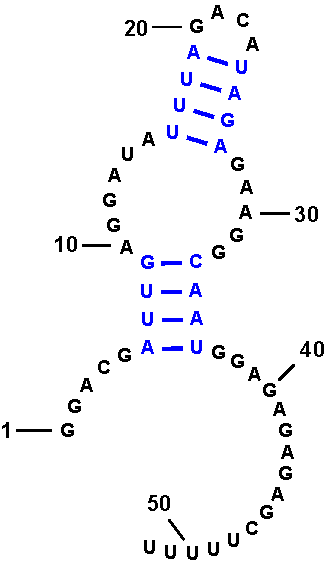
\includegraphics[scale=0.3]{figs/TBWN-B-4}}
&
  %\hspace{-0.5cm}
\hspace{-0.3cm}\raisebox{2.cm}{\mtwo{{\raisebox{4.5cm}{\panel{C}} \hspace{-0.3cm} 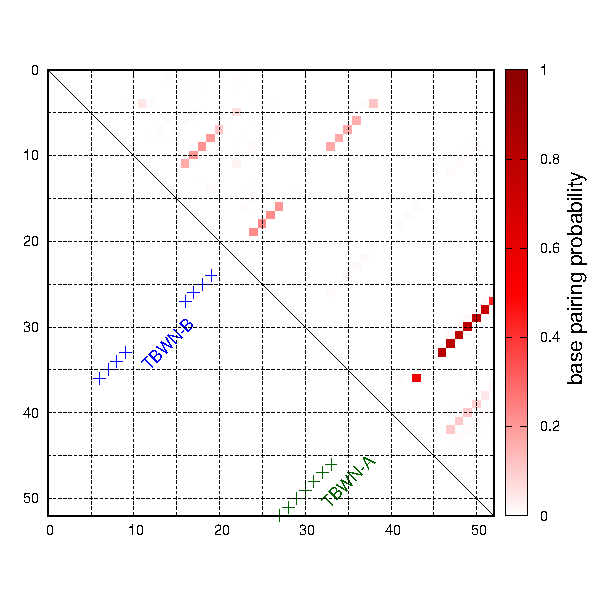
\includegraphics[scale=0.5]{figs/heatmap_fig1A}}}}
\\[0.2cm]
%\hspace{-1cm}
% 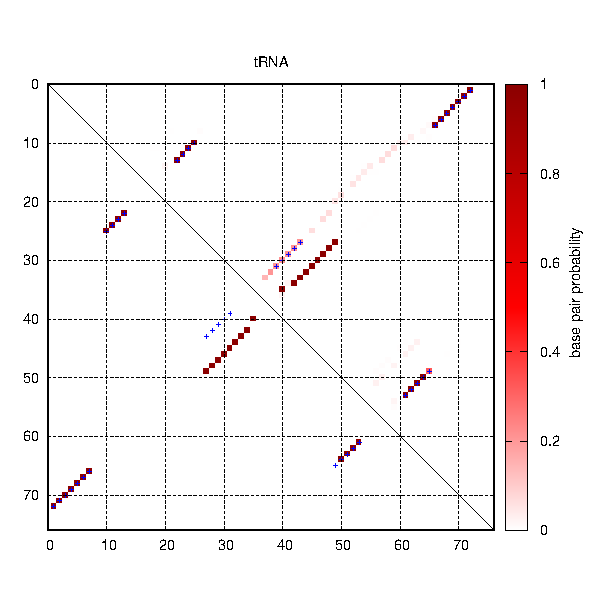
\includegraphics[scale=0.4]{figs/tRNA_heatmap_dark}
\end{tabular}
\\[0.2cm]
\panel{D}
\\[-0.2cm]
%\centering
  \begin{tabular}{@{}c@{ }|@{}c@{ }|l@{\!}c@{ }|l@{\!}c@{}}
    & \ span & \multicolumn{2}{c|}{minimum free energy} & \multicolumn{2}{c}{partition-function} \\
    \hline
    bottom-up, {\em exact} &$\infty$ &    Zuker\cite{zuker+stiegler:1981} & $O(n^3)$ & McCaskill\cite{mccaskill:1990} & $O(n^3)$ \\    
    \hline
    \mtwo{local folding} & \mtwo{$L$}  &  \mtwo{Localfold\cite{lange+:2012}} & \mtwo{$O(nL^2)$} & {RNAplfold\cite{bernhart+:2006}} & \mtwo{$O(nL^2)$}\\
                  &           &   &       &   Rfold\cite{kiryu+:2008}        &\\
    \hline    
    left-to-right, {\em exact}  & \mtwo{$\infty$} & \mtwo{\linearfold\cite{huang+:2019}} & $O(n^3)$  & \mtwo{\linearpartition} & $O(n^3)$\\
     \quad + {\em beam pruning} &     && $O(n b\log b)$ && $O(n b^2)$
    %% left-to-right & \mtwo{\linearfold, $O(n b\log b)$} & \linearpartition, $O(n b^2)$\\[-0.1cm]
    %% + {\em beam pruning} & 
  \end{tabular}
  %% \caption{Comparison between classical, local, and left-to-right algorithms for MFE and partition function calculation. 
  %%   \linearfold and \linearpartition enjoy linear runtime thanks to left-to-right order which enables heuristic beam pruning,
  %%   and both become exact $O(n^3)$ algorithms without pruning. % size $b$ is $+\infty$.
  %%   ``Span'' denotes the maximum pair distance allowed ($\infty$ means no limit);
  %%   it is a small constant in local methods (e.g., default $L$=70 in RNAplfold).
  %%   \label{tab:overall}
  %% } 
\caption{
  %An example % of Tebowned RNA
%  illustrates 
% some RNAs 
  %that
  An RNA can fold into multiple structures at equilibrium.
  {\bf A--B}:~Two 
  %such 
  secondary structures of Tebowned RNA: TBWN-A and TBWN-B~\cite{Cordero+Das:2015}.
{\bf C}: upper triangle shows the estimated base pairing probability matrix for this RNA using \viennarnafold,
where darker red squares represent higher probility base pairs;
the lower triangle shows the two different structures; %TBWN-A and TBWN-B  %(in green)  (in blue),
%at equilibrium;
%(green crosses for TBWN-A and blue for TBWN-B base pairs);
    %    {\bf C}: TBWN-B secondary structure.
{\bf D:} Comparison between classical, local, and left-to-right algorithms for MFE and partition function calculation. 
    \linearfold and \linearpartition enjoy linear runtime because of a left-to-right order that  enables heuristic beam pruning,
    and both become exact $O(n^3)$ algorithms without pruning. % size $b$ is $+\infty$.
    ``Span'' denotes the maximum pair distance allowed ($\infty$ means no limit);
    it is a small constant in local methods (e.g., default $L$=70 \nts in RNAplfold).
\label{fig:overview}}
\vspace{-0.3cm}
\end{figure}
